% TODO: Explaination of the syntatic algorithm
% TODO: Perhaps some more (or more detailed) benchmarking 
\documentclass[a4paper,notitlepage]{scrartcl}

\usepackage{amsmath}
\usepackage{amssymb}
\usepackage{minted}
\usepackage[margin=2cm]{geometry}
\usepackage[final]{pdfpages}

% Use the nicer phi
\let\phi\varphi

\title{Conjunctive Normal Form}
\author{Bill Noble\\ Tim van der Molen}
\date{January 2014}

\begin{document}
\maketitle

\section{Introduction}

A formula is in conjunctive normal form (CNF) if it is a conjunction of
subformulas, each of which either is a literal (i.e. an atom or the negation of
an atom) or a disjunction of literals.
As a special case, a CNF formula may consist of only one conjunct, in which
case it simply is either a literal or a disjunction of literals. 
CNF is very useful in automatic theorem proving, because its structure allows
for efficient formula evaluation.
In this report we discuss and compare two algorithms to transform arbitrary
propositional formulas into CNF.
The first algorithm employs syntactical manipulation while the second has a
semantical approach relying on truth tables.
The two algorithms have been implemented in the Python programming language.

\section{Formula Representation}

We use tuples and lists to represent formulas in Python.
As may be expected, tuples in Python are enclosed in round brackets while lists
are enclosed in square brackets.
The elements of a tuple or a list are separated by commas.
For example, \texttt{(a, b, c)} is a tuple and \texttt{[a, b, c]} is a list.
More specifically, a formula representation is recursively defined as follows.

\begin{enumerate}

\item
If \texttt{s} is a string, then \texttt{(s,)} is a formula.

\item
If \texttt{f} is a formula, then \texttt{('not', f)} is a formula.

\item
If \texttt{f} and \texttt{g} are formulas, then \texttt{('arrow', f, g)} is a
formula.

\item
If \texttt{f}$_1$, $\ldots$, \texttt{f}$_n$ are formulas, then \texttt{('and',
[f$_1$, $\ldots$, f$_n$])} is a formula.

\item
If \texttt{f}$_1$, $\ldots$, \texttt{f}$_n$ are formulas, then \texttt{('or',
[f$_1$, $\ldots$, f$_n$])} is a formula.
\end{enumerate}

\noindent
For example, the formula $p \land \lnot q \land (r \to s)$ is represented as
\texttt{('and', [('p',), ('not', ('q',)), ('arrow', ('r',), ('s',))])}.

\section{The Syntactic Algorithm}

The syntactic CNF algorithm exploits the distributivity of disjunction over
conjunction to transform formulas into CNF.
For example, the non-CNF formula $\phi \lor (\psi \land \chi)$ may be
transformed into the logically equivalent CNF formula $(\phi \lor \psi) \land
(\phi \lor \chi)$ by distributing disjunctions over conjunction.

The syntactic CNF algorithm is applicable only to formulas that are in negation
normal form (NNF).
A formula is in NNF if only atoms are negated and the only other logical
operators that occur in it are disjunction and conjunction.
Therefore, in order for a formula to be transformed into CNF, it first must
have been transformed into NNF.

The NNF algorithm, in turn, is applicable only to formulas in which negation,
disjunction and conjunction occur as the only operators.
Hence, every implicative subformula of the form $\phi \to \psi$ must be
transformed into an equivalent disjunction of the form $\lnot\phi \lor \psi$.
This is done by the impl\_to\_disj() function, which may be defined as follows.

\begin{enumerate}

\item
If $\phi$ is an atom, then $\mathrm{impl\_to\_disj}(\phi) = \phi$.

\item
If $\phi = \lnot\psi$, then $\mathrm{impl\_to\_disj}(\phi) =
\lnot\mathrm{impl\_to\_disj}(\psi)$.

\item
If $\phi = \psi \to \chi$, then $\mathrm{impl\_to\_disj}(\phi) =
\lnot\mathrm{impl\_to\_disj}(\psi) \lor \mathrm{impl\_to\_disj}(\chi)$.

\item
If $\phi = \psi_1 \land \ldots \land \psi_n$, then
$\mathrm{impl\_to\_disj}(\phi) = \mathrm{impl\_to\_disj}(\psi_1) \land \ldots
\land \mathrm{impl\_to\_disj}(\psi_n)$.

\item
If $\phi = \psi_1 \lor \ldots \lor \psi_n$, then
$\mathrm{impl\_to\_disj}(\phi) = \mathrm{impl\_to\_disj}(\psi_1) \lor \ldots
\lor \mathrm{impl\_to\_disj}(\psi_n)$.

\end{enumerate}

\noindent
The Python implementation is as follows.

\begin{minted}[frame=single]{python}
def impl_to_disj(f):
    if atom(f):
        return f
    if f[0] == 'not':
        return ('not', impl_to_disj(f[1]))
    if f[0] == 'or' or f[0] == 'and':
        return (f[0], [impl_to_disj(g) for g in f[1]])
    if f[0] == 'arrow':
        return ('or', [('not', impl_to_disj(f[1])), impl_to_disj(f[2])])
    else:
        raise ValueError('unknown operator:', f[0])
\end{minted}

\noindent
The atom() function returns true if its tuple argument contains exactly 1
argument and false otherwise:

\begin{minted}[frame=single]{python}
def atom(f):
    return len(f) == 1
\end{minted}

The nnf() function may be defined as follows.

\begin{enumerate}

\item
If $\phi$ is an atom, then $\mathrm{nnf}(\phi) = \phi$.

\item
If $\phi = \lnot\psi$, then:

\begin{enumerate}

\item
If $\psi$ is an atom, then $\mathrm{nnf}(\phi) = \phi$.

\item
If $\psi = \lnot\chi$, then $\mathrm{nnf}(\phi) = \mathrm{nnf}(\chi)$.

\item
If $\psi = \chi_1 \land \ldots \land \chi_n$, then $\mathrm{nnf}(\phi) =
\mathrm{nnf}(\lnot\chi_1) \lor \ldots \lor \mathrm{nnf}(\lnot\chi_n)$.

\item
If $\psi = \chi_1 \lor \ldots \lor \chi_n$, then $\mathrm{nnf}(\phi) =
\mathrm{nnf}(\lnot\chi_1) \land \ldots \land \mathrm{nnf}(\lnot\chi_n)$.

\end{enumerate}

\item
If $\phi = \psi_1 \land \ldots \land \psi_n$, then $\mathrm{nnf}(\phi) =
\mathrm{nnf}(\psi_1) \land \ldots \land \mathrm{nnf}(\psi_n)$.

\item
If $\phi = \psi_1 \lor \ldots \lor \psi_n$, then $\mathrm{nnf}(\phi) =
\mathrm{nnf}(\psi_1) \lor \ldots \lor \mathrm{nnf}(\psi_n)$.

\end{enumerate}

\noindent
The Python implementation is as follows.

\begin{minted}[frame=single]{python}
def nnf(f):
    return nnf_do(impl_to_disj(f))

def nnf_do(f):
    if atom(f):
        return f
    if f[0] == 'not':
        if atom(f[1]):
            return f
        if f[1][0] == 'not':
            return nnf_do(f[1][1])
        if f[1][0] == 'and':
            return ('or', [nnf_do(('not', g)) for g in f[1][1]])
        if f[1][0] == 'or':
            return ('and', [nnf_do(('not', g)) for g in f[1][1]])
        else:
            raise ValueError('unexpected operator:', f[1][0])
    if f[0] == 'and' or f[0] == 'or':
        return (f[0], [nnf_do(g) for g in f[1]])
    else:
        raise ValueError('unexpected operator:', f[0])
\end{minted}

The $\mathrm{cnf}()$ function is defined as follows.

\begin{enumerate}

\item
If $\phi$ is a literal, then $\mathrm{cnf}(\phi) = \phi$.

\item
If $\phi = \psi_1 \land \ldots \land \psi_n$, then $\mathrm{cnf}(\phi) =
\mathrm{cnf}(\psi_1) \land \ldots \land \mathrm{cnf}(\psi_n)$.

\item
If $\phi = \psi_1 \lor \ldots \lor \psi_n$, then $\mathrm{cnf}(\phi) =
\mathrm{dist}(\mathrm{cnf}(\psi_1), \mathrm{cnf}(\psi_2 \lor \ldots \lor
\psi_n))$.

\end{enumerate}

\noindent
The $\mathrm{dist}()$ function performs the disjunction distribution and is
defined as follows.

\begin{enumerate}

\item
If $\phi = \chi_1 \land \ldots \land \chi_n$, then $\mathrm{dist}(\phi, \psi) =
\mathrm{dist}(\chi_1, \psi) \land \ldots \land \mathrm{dist}(\chi_n, \psi)$.

\item
If $\psi = \chi_1 \land \ldots \land \chi_n$, then $\mathrm{dist}(\phi, \psi) =
\mathrm{dist}(\phi, \chi_1) \land \ldots \land \mathrm{dist}(\phi, \chi_n)$.

\item
Otherwise, $\mathrm{dist}(\phi, \psi) = \phi \lor \psi$.

\end{enumerate}

\noindent
The algorithm may be described as follows.
It starts at the deepest nested conjunctions and, if necessary, applies the
distribution rule.
This moves the original conjunctions up one level in the formula.
At this level distribution is applied again, if necessary.
This process is continued until all conjunctions have been pushed up above any
disjunction.

The Python implementation of $\mathrm{cnf}()$ and $\mathrm{dist}()$ is as
follows.

\begin{minted}[frame=single]{python}
def cnf(f):
    if atom(f) or f[0] == 'not':
        return f
    if f[0] == 'and':
        return ('and', [cnf(g) for g in f[1]])
    if f[0] == 'or':
        if len(f[1]) == 0:
            return f
        if len(f[1]) == 1:
            return cnf(f[1][0])
        else:
            return dist(cnf(f[1][0]), cnf(('or', f[1][1:])))
    else:
        raise ValueError('unknown operator:', f[0])

def dist(f, g):
    if f[0] == 'and':
        if len(f[1]) == 0:
            return f
        else:
            return ('and', [dist(h, g) for h in f[1]])
    if g[0] == 'and':
        if len(g[1]) == 0:
            return g
        else:
            return ('and', [dist(f, h) for h in g[1]])
    else:
        return ('or', [f, g])
\end{minted}

After a formula has been transformed into CNF, it may contain nested lists of
conjunctions and disjunctions.
These lists are flattened or collapsed by the flatten() function.
As a final step, the remove\_dups() function removes from every disjunction
list duplicate disjuncts and likewise for the conjunction list.

The Python implementation for these functions is as follows.

\begin{minted}[frame=single]{python}
def flatten(f):
    if f[0] == 'and':
        return ('and', flatten_conj(f[1]))
    if f[0] == 'or':
        return ('or', flatten_disj(f[1]))
    else:
        return f

def flatten_conj(flist):
    if flist == []:
        return flist
    if flist[0][0] == 'and':
        return flatten_conj(flist[0][1] + flist[1:])
    else:
        return [flatten(flist[0])] + flatten_conj(flist[1:])

def flatten_disj(flist):
    if flist == []:
        return flist
    if flist[0][0] == 'or':
        return flatten_disj(flist[0][1] + flist[1:])
    else:
        return [flist[0]] + flatten_disj(flist[1:])

def remove_dups(f):
    if f[0] == 'and':
        flist = []
        for g in f[1]:
            g = remove_dups(g)
            if not g in flist:
                flist.append(g)
        return ('and', flist)
    if f[0] == 'or':
        return ('or', list(set(f[1])))
    else:
        return f
\end{minted}

\noindent
To incorporate these functions into the function chain, the original cnf()
function is renamed to cnf\_do() and the new cnf() function is as follows.

\begin{minted}[frame=single]{python}
def cnf(f):
    return remove_dups(flatten(cnf_do(nnf(f))))
\end{minted}

\section{The Semantic Algorithm}

Rather than converting $f$ to CNF directly, the $cnf\_tt$ algorithm
        constructs a truth table and uses it to produce a formula in CNF
        that is logically equivalent to $f$ (i.e. it is true at exactly
        the rows where $f$ is true). 
It is more intuitive to use this strategy to produce a formula
        in DNF.

\begin{displaymath}
\begin{array}{|c|c|c|c}
   p
 & q
 & r
 & (p\lor{}q)\rightarrow{}r \\
\hline
0 & 0 & 0 & 1 \\
0 & 0 & 1 & 1 \\
0 & 1 & 0 & 0 \\
0 & 1 & 1 & 1 \\
1 & 0 & 0 & 0 \\
1 & 0 & 1 & 1 \\
1 & 1 & 0 & 0 \\
1 & 1 & 1 & 1 \\
\hline
\end{array}
\end{displaymath}

To write a formula that is true at exactly one row in a truth table
        (i.e. it is true there and nowhere else), one 
        takes the conjunction of all the literals or their negations depending
        on their truth or falsity at that row.
For example, the formula $\land [\lnot p, q, r]$ is true at exactly row $4$ in
        the truth table above.
Reading a DNF formula from a truth table is an extension of this idea:
        just take the disjunction of such formulas for each row where $f$
        is true.
The resulting formula is in DNF and is true at exactly the lines where $f$
        is true (i.e. it is logically equivalent).
Thus we have:
\[
\lor[p,q]\rightarrow r \equiv 
\lor [
\land[\lnot p, \lnot q,\lnot r], 
\land[\lnot p,\lnot q,r], 
\land[\lnot p,q,r], 
\land[p,\lnot q,r], 
\land[p,q,r]
     ]
\]
        
\begin{minted}[frame=single]{python}
# Uses the truth table method to compute disjunctive normal form
def dnf_tt(f):
    # filter the truth table to only rows where f is True
    f_true_tt = [row for row in gen_tt(get_atoms(f)) 
                 if evaluate(f, row) == True]
    # return an 'or' list of 'and' lists (one for each row in
    # f_true_tt) such that each 'and' list contains p when
    # p is True in the row and ('not', p) when it is False.
    return tuple(['or', [tuple(['and', 
        [p if row[p] else tuple(['not', p]) for p in row.keys() ]]) 
        for row in f_true_tt] ])
\end{minted}

To read the CNF from the truth table, we take the opposite (but obviously
        logically equivalent) approach: the goal is to write a formula
        that is false at exactly the lines where $f$ is false. 
Say we wanted to write a formula that is false at exactly line $3$.
The formula $\land[\lnot p, q, \lnot r]$ is true at exactly line $3$, so its
        negation is false exactly there.
Applying the De Morgan's rule gives $\lor[p, \lnot q, r]$.
Naturally, taking the conjunction of such formulas, we can pick out more rows.
Thus we have:
\[
\lor[p,q]\rightarrow r \equiv 
\land[
\lor[p, \lnot q, r], 
\lor[\lnot p, q, r], 
\lor[\lnot p, \lnot q, r], 
     ]
\]

\begin{minted}[frame=single]{python}
# Uses the truth table method to compute conjunctive normal form
def cnf_tt(f):
    # filter the truth table to only rows where f is False 
    f_false_tt = [row for row in gen_tt(get_atoms(f)) 
                  if evaluate(f, row) == False]
    # return an 'and' list of 'or' lists (one for each row in
    # f_false_tt) such that each 'or' list contains ('not', p) when
    # p is True in the row and p when it is False.
    return tuple(['and', [tuple(['or', 
        [p if not row[p] else tuple(['not', p]) for p in row.keys()] ]) 
        for row in f_false_tt]])
\end{minted}

\section{Analysis}

The $cnf\_tt$ algorithm has a higher up-front cost than $cnf$.
The cost of generating the empty truth table is relatively small; 
It is a list of the $2^n$ possible valuations (where $n$ is the
        number of atomic propositions):
\begin{minted}[frame=single]{python}
# Generates all possible valuations for a given set of atoms.     
def gen_tt(atoms):
    from itertools import product
    return [{p:val for (p, val) in zip(atoms, vals)} for vals in 
         product([False, True], repeat=len(atoms))]
\end{minted}
Filtering the truth table to only the rows where $f$ is $False$ is rather
        intensive since the formula must be evaluated at each of the
        $2^n$ rows and the evaluation function may be called up to once
        for each subformula of $f$.
Nevertheless, $cnf\_tt$ performs better on longer random formulas, especially 
        where total number of propositions greatly exceeds the total number of
        unique propositions. 

Below: time difference ($cnf$ minus $cnf\_tt$) in converting $5000$ random formulas
        to CNF.
The $x$ axis ranges over the number of unique propositions, and the $y$ axis 
        is the total number of propositions in the formula.\\

\noindent
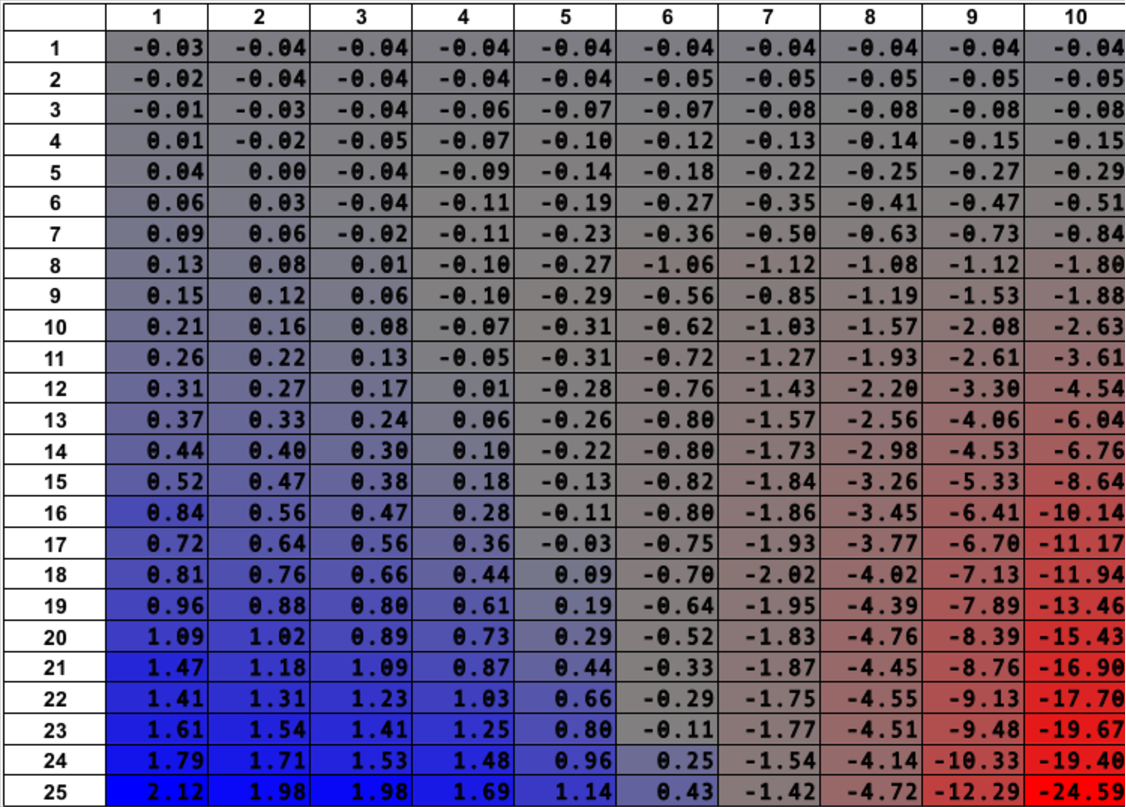
\includegraphics[
    page=1,
    width=\textwidth,
    height=\textheight,
    keepaspectratio
]{report_colors_cropped.pdf}
\vfill
\newpage

For formulas given in DNF, $cnf\_tt$ is faster for formulas of any length 
        sentences, and $cnf$ reaches Python's default maximum recursion depth 
        of $1000$ beginning at $3$ propositions.

The run time of $cnf$ is agnostic to the number of unique propositions
        in the given formula since uniqueness of a proposition is primarily
        semantic notion.
The semantic algorithm, $cnf\_tt$, is less concerned with the syntactic
        structure of the given formula since this has less bearing on the
        construction of a truth table.
The relative strengths of the two algorithms highlights two distinct ways that
        a propositional formula can be complex.
\end{document}
